\section{Conclusions and Future Work}\label{sec_conclusion}
We presented safety-critical software allocation on a network of heterogeneous computing units, with respect to failure rate, processor speed and power specification. The applications are developed according to the AUTOSAR standard and possess timing and reliability requirements. We assume worst-case response time analysis and age delay analysis to compute the schedulability of tasks and chains, respectively, which are exact but complex timing analysis techniques. Furthermore, the allocation considers maximization of reliability to meet the reliability requirements of the safety-critical applications via fault tolerance. The latter exerts computational overhead especially on the delay calculation, and requires more computational resources and consumes more power.

We proposed hybrid particle-swarm optimization algorithms to optimize the power total consumption of the distributed safety-critical software applications while meeting the requirements. The hybridization algorithms comprise differential evolution, hill climbing and stochastic hill climbing. For comparison, we also included differential evolution and local particle-swarm optimization algorithms. The result of the algorithms are compared to \ilp{} results in the small and medium software allocations. In general, the the hybridization with the hill-climbing algorithms performed better than the other meta-heuristic algorithms. The hybridization with the stochastic hill-climbing performed well in the largest optimization problem.

In future work, we plan to consider a complex power model that relates load to heat dissipation and the effect on reliability over a long run. The current work is limited to offline configuration, however, it can be extended to address the need for re-configurable distributed system, e.g., in the case of software evolution, system failures .

\subsubsection*{Acknowledgement}
This work is supported by the Swedish Governmental Agency for Innovation Systems (Vinnova) through the VeriSpec project, and the Swedish Knowledge Foundation (KKS) through the projects HERO and DPAC.

\pagebreak
% Biography Section
%\section*{ }
% \noindent \textbf{Author1 name} author description goes here.
% \subsection*{  } % This subsection (with no heading) is added to give more space between two biographies
% \noindent \textbf{Author2 name}  author description goes here. 

% \authorbiography[scale=0.3,overhang=0pt,wraplines=9,imagewidth=3cm,imagepos=l,yearofbirth={1887},yearofdeath={1961}]{nesredin.jpg}{Nesredin Mahmud}
% {\blindtext}%

% \authorbiography[scale=0.3,wraplines=10,overhang=0pt,imagewidth=5cm,imagepos=r,yearofbirth={1564},yearofdeath={1616}]{guillermo.jpg}{Guillermo Rodriguez-Navas}{\blindtext}%

% \authorbiography[scale=0.2,width={4cm},imagewidth=6cm,wraplines=15,imagepos=l,overhang=0pt,yearofbirth={1879},yearofdeath={1955}]{hamid.jpg}{Hamid Reza Faragardi}{\blindtext}%

% \authorbiography[scale=0.1,imagewidth=3cm,wraplines=10,imagepos=r,overhang=0pt,yearofbirth={1879},yearofdeath={1955}]{saad.jpg}{Saad Mubeen}{\blindtext}%

% \authorbiography[scale=0.1,imagewidth=3cm,wraplines=10,imagepos=r,overhang=0pt,yearofbirth={1879}]{cristina.jpg}{Cristina Seceleanu}{\blindtext}%


% \Authorbiography% Standard behaviour


% \Authorbiography[totoc=true,BiographyName={Authors}] % Use some more configurability


\par\noindent 
\parbox[t]{\linewidth}{
\noindent\parpic{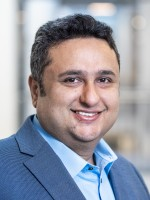
\includegraphics[height=1.5in,width=1in,clip,keepaspectratio]{images/authors/saad.jpg}}
\noindent {\bf Saad Mubeen}\
Dr. Mubeen is an Associate Professor at Mälardalen University, Sweden. He has previously worked in the vehicle industry as a Senior Software Engineer at Arcticus Systems and as a Consultant for Volvo Construction Equipment, Sweden. Dr. Mubeen is a Senior Member of IEEE. He is a Co-chair of the Subcommittee on In-vehicle Embedded Systems within the IES Technical Committee on Factory Automation. His research focus is on model- and component-based development of predictable vehicle software, modeling and timing analysis of in-vehicle communication, and end-to-end timing analysis of distributed embedded systems. Within this context, he has co-authored over 125 publications in peer-reviewed international journals, conferences and workshops. He has received several awards, including the IEEE Software Best Paper Award in 2017. He is a PC member and referee for several international conferences and journals respectively. He is a guest editor of IEEE Transactions on Industrial Informatics (TII). He has co-organized several special sessions at the international conferences such as IEEE IECON and ICIT.  He has also organized the 9th International Workshop on Compositional Theory and Technology for Real-Time Embedded Systems (CRTS 2016) and Model-based Engineering of Cyber Physical Systems track at the 13th International Conference on Information Technology: New Generations (ITNG), 2016.}
\vspace{4\baselineskip}